%!TEX root =  testMain.tex

\chapter[Appendix]{Appendix}
\section{Background on probabilities - the meaning of random variables}

Bayesian Networks consists of nodes, and arcs between those nodes. The nodes in a Bayesian Network are random variables. But what are random variables? The following explanation is adapted from \citep{Jaeger2019}.

A random variable (RV) is not just a natural language statement, but it's a mathematical object. It is a function or mapping of the form $X : \Omega \rightarrow S$, where $\Omega$ is the universe, and $S$ is the sample space. The RV maps some elementary event in the universe, to a specific output in sample space (Figure~).


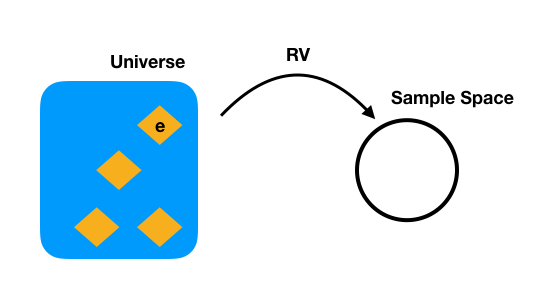
\includegraphics[width=\linewidth]{images/rv1.png}


This is not really an explanation, because 1) what is a universe? 4) what is a sample space? 3) mapping how? 2) what is an elementary event? and so on.

The universe can be super abstract. It is the place where the events happen that we're interested in. It can be our actual universe, a simulation, or a subset or our actual universe or simulation. Elementary events are the events that happen within our universe - they are the elements of the set that is the universe. A random variable is a procedure, with a method, that can map an event to a certain value. All the possible values that an event can take, are collected in the sample space S. \footnote{This is how far I'll go with this explanation, if you want to know about $\sigma$-fields I don't have time to understand and explain all of that. And I don't think its necessary for the problems with bayesian networks.}

To illustrate this, we have a simple example (Example~1).


\begin{example}
Let's say that we are observing a painter who wants to put down the first layer of paint on their canvas. The painter has to pick the color of the background layer. $\Omega$ is the universe, and contains all events where this painter is picking a color for a background for an oil painting. $\S$ is the sample space, and is the set of all colors that the painter can pick. The RV $X$ maps events to values in sample space. For this initial simple example, $S = \{green, blue, orange\}$. Then $X^{-1}(orange)$ refers to the set of all events where the painter picked "orange" as the background color.

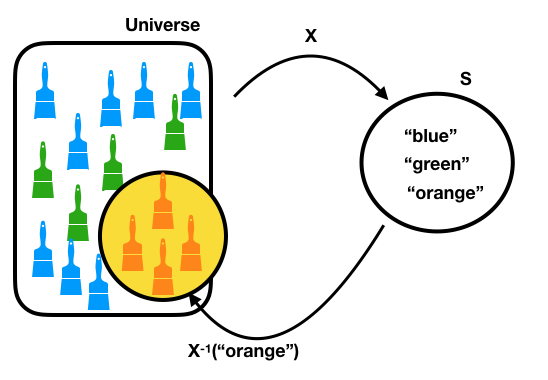
\includegraphics[width=\linewidth]{images/rv2.png}
\end{example}

In our example, we say that the RV $X$ maps events to values in sample space (and inversely, $X^{-1}$ maps a value in sample space to a set of events). However, how does this mapping work? The mapping itself is not a mathematical object (eg, we don't do $X(\omega) = 2*\omega^2 = "orange"$). Instead, we observe a certain event $w$ in $\Omega$, and measure in some way, to find out what value $w$ takes in $S$. For things like dice-rolls, it is clear how we observe the event (we just look at it), just like in our painting example. However, there are several ways that we can observe and map this situation, operationalise it, which all respond to different RV's:

\begin{enumerate}
\item \textbf{RGB Color-picker}: we take a picture of the canvas, and analyse it in the computer. We have selected certain ranges of RGB values that correspond to orange, blue and green, respectively. The average color of the canvas within one of the RGB-color bins is how we know what color it is.
\item \textbf{Taste}: we have a super-taster who specialises in paint pigments \footnote{Not the healthiest of occupations.}. When she blind-tastes a bit of the paint, she can tell us what color it is, because the pigment that causes the color orange tastes different from the green, which tastes different from blue.
\item \textbf{Subjective taste}: I have my own opinions on whether some paint color is orange, blue or green. I see the canvas, and I decide \footnote{I might be colorblind}.
\item Think of something else ridiculous.
\end{enumerate}

Of these operationalisations of the RV you can think many things. Some might be more valid than others. We can only know if we trust the final probability assignment (I will get there in a second) if we can agree with the method of mapping - which is the random variable. The operationalisation of the random variable is a big deal, and to know if it is valid/accurate, we need to know exactly how it was mapped, because then we can argue about it if we don't like it.

Now, let's assume we have some sort of way of determining the color of the canvas (really does not matter which one, as long as we pick one). Then, we can talk about probability! Probability maps an event to a real number $[0, 1]$. The `event' here is not the same as an elementary event. Instead, `event' means that a RV takes some value in the sample space - so an event is the set of elementary events in the universe, for which the random variable on that event takes a specific value - $\{\omega \in \Omega \vert X(\omega) \in orange\}$ is the set of cases where the color on the canvas is orange.

Then, we can assign a probability value to this event, simply $P(X \in A) = p$. There's a whole debate on what $p$ should actually mean - is it a degree of belief, or a frequency, or something else? The frequentist view is that we repeat measurements - eg, we apply the RV a lot (every time the painter is starting a new painting), and count how often the canvas is orange, and then divide that by the total amount of new canvases started, and this should be the value of $p$.  In the subjectivist view, $p$ can be any value as long as that value reflects our belief on how many times the painter paints orange vs blue vs green backgrounds. Then, we have our probability! 

A different problem is for our universe. Are we only counting oil paintings, or are we also counting acrylics. Or did we say `painting' when we meant `artwork' and should we also take the painter's sketches and pastel drawings into account? This is the second problem, and it is known as the problem of the reference class. Different reference classes will result in different frequencies (also in different degrees of belief). That's why it is not just important to specify operationalisations for every random variable, but also specify exactly what part of the universe you're investigating (eg, what is and isn't in $\Omega$).


